\ifSTANDALONE
\section{Encoder \& Drehzahlgeber}
\fi
\ifEMBED
\subsection{Encoder \& Drehzahlgeber}
\fi

Die vorgesehenen Motorfunktionen verlangen lediglich beim Brushlessmotor
nach einem Feedback über die Rotation des Motors, da der Schrittmotor
definiert und feingranuliert betrieben wird und der Gleichstrommotor
keinerlei Ansprüche stellt weder an Drehzahl noch an Position.

Encoder sind relativ teuer und der Einsatz des Brushlessmotors verlangt
lediglich nach einem Feedback zur Rotation bzw. Winkelgeschwindigkeit.
Die absolute oder relative Position ist für die Anwendung nicht von
Bedeutung. Somit lässt sich ein einfaches Feedback vorsehen für die
Regelung der Drehzahl mittels optischer oder magnetischer Elemente.
\ifSTANDALONE
\begin{figure}[h!]
	\centering
	\begin{tikzpicture}
		% Koordinaten
		\draw[->] (-0.5, 0) -- (8, 0) node[anchor=north] {$t$};
		\draw[->] (0, -1.5) -- (0, 3) node[anchor=east] {$u,\varphi$};
		% Rotation
		\draw[blue] (0,0) sin (1,1) cos (2,0) sin (3,-1) cos (4,0)
			sin (5,1) cos (6,0) sin (7,-1)
			node[right] {$\varphi$};
		% Signal
		\draw[-, thick, red]
			(0,0) -- (0.8,0) -- (0.8,2) -- (1.2,2) -- (1.2,0) -- 
			(4.8,0) -- (4.8,2) -- (5.2,2) -- (5.2,0) -- (7.5,0);
		% Messung
		\draw[<->] (0.8,1.5) -- (4.8,1.5) node[midway, above] {$t_{r}$};
	\end{tikzpicture}
	\caption{Vereinfachtes Puls-Feedback eines Hall-Effekt-Scahlters}
	\label{fig:hall-effekt-schalter}
\end{figure}
\fi
\ifEMBED
\begin{figure}[h!]
	\centering
	\begin{tikzpicture}
		% Koordinaten
		\draw[->] (-0.5, 0) -- (8, 0) node[anchor=north] {$t$};
		\draw[->] (0, -1.5) -- (0, 3) node[anchor=east] {$u,\varphi$};
		% Rotation
		\draw[blue] (0,0) sin (1,1) cos (2,0) sin (3,-1) cos (4,0)
			sin (5,1) cos (6,0) sin (7,-1)
			node[right] {$\varphi$};
		% Signal
		\draw[-, thick, red]
			(0,0) -- (0.8,0) -- (0.8,2) -- (1.2,2) -- (1.2,0) -- 
			(4.8,0) -- (4.8,2) -- (5.2,2) -- (5.2,0) -- (7.5,0);
		% Messung
		\draw[<->] (0.8,1.5) -- (4.8,1.5) node[midway, above] {$t_{r}$};
	\end{tikzpicture}
	\caption{Vereinfachtes Puls-Feedback eines Hall-Effekt-Scahlters}
	\label{fig:hall-effekt-schalter}
\end{figure}
\fi
Als optisches Messisnturment kann eine Lichtschranke mit 
Reflexionsstriefen oder Löchern eingesetzt werden. Diese verlangen
nur nach einer geringfügigen Modifikation des Rotierenden Körpers und
sind relativ günstig. Optische Messtechnik hat den Nachteil, dass
Störungen relativ leicht in die Messung einfliessen können, was fatale
Folgen für die Regelung hat. Magnetische Messinstrumente sind gegenüber
Störungen deutlich resistenter, da hierfür starke Magnetfelder benötigt
werden, welche so nicht einfach auftreten. Der Einsatz solcher Messtechnik
verlangt jedoch nach einer Modifikaiton der Mechanik, da Magnete in den
rotierenden Körper einebaut werden müssen. Dies birgt ein gewisses
Risiko für mechanische Unwucht des Rotationskörpers.

\ifSTANDALONE
\subsection{Magnetischer Drehzahlgeber}
\fi
\ifEMBED
\subsubsection{Magnetischer Drehzahlgeber}
\fi
Um einen eigenen magnetischen Drehzahlgeber zu erstellen wird ein
sog. Hall-Effekt-Schalter eingesetzt. Dieser reagiert mit seinem Ausgang
auf ein auftretendes Magnetfeld. Das Gegenstück zum Hall-Effekt-Schalter
ist ein Magnet, welcher in das rotierende Objekt eingebaut wird. Aus 
mechanischen Gründen, wie etwa der Unwucht, werden typisch 2 Magnete
oder ein Vielfaches davon in den rotierenden Körper eingebaut.

Bei der Rotation des Körpers entstehen durch das Vorbeigehen der Magnete
am Hall-Effekt-Schalter Impulse. Aus diesen Impulsen lässt sich mittels einer
Zeitmessung direkt die Drehzahl bestimmen. Die Abbildung 
\ref{fig:hall-effekt-schalter} illustriert das Prinzip anhand eines
Beispiels mit einem Magneten am Rotationskörper.
%
\ifSTANDALONE
\begin{figure}[h!]
	\centering
	\includegraphics[width=0.75\textwidth]{../src/Bilder/AH180N_functional.png}
	\caption{Funktionelles Blockschaltbild des Hall-Effekt-Scahlters AH180N}
	\label{fig:AH180N_functional}
\end{figure}
\fi
%
\ifEMBED
\begin{figure}[h!]
	\centering
	\includegraphics[width=0.75\textwidth]{./src/Bilder/AH180N_functional.png}
	\caption{Funktionelles Blockschaltbild des Hall-Effekt-Scahlters AH180N}
	\label{fig:AH180N_functional}
\end{figure}
\fi
%
Ein solches Verfahren lohnt sich bei schnellen Winkelgeschwindigkeiten
und ist für diesen Anwendungsfall sehr effizient. Zugehörige
Hall-Effekt-Schalter lassen sich einfach montieren und sind gegen Störungen
sehr robust. Ein mögliches Modell für einen Hall-Effekt-Schalter ist der
AH180N. Dieser bietet einen Open-Drain Ausgang welcher somit logische Pegel
liefert (siehe Abbildung \ref{fig:AH180N_functional}). Interessant ist diese
Art von Drehzahl-Geber insbesondere durch ihren geringen Preis, denn solche
Hall-Effekt-Schalter wie der AH180N befinden
sich im Preissegment < 1 CHF.
